\documentclass[a4paper,conference]{IEEEtran}
\usepackage{amsmath,amssymb,booktabs,graphicx}
\usepackage[hidelinks]{hyperref}
\hypersetup{pdftitle={Retinal Vessel Segmentation with Study Group Learning},
pdfauthor={Prerak Arya and Abhsihek Meena},
pdfsubject={Computer vision project report and paired DRIVE pilot}}
\graphicspath{{figures/}}
\title{Retinal Vessel Segmentation on DRIVE:\\
A Paired Evaluation of Study Group Learning}
\author{\IEEEauthorblockN{Prerak Arya}
\IEEEauthorblockA{230039}
\and
\IEEEauthorblockN{Abhsihek Meena}
\IEEEauthorblockA{230137}}

\begin{document}
\maketitle
\begin{abstract}
Retinal vessel segmentation is difficult when annotated data are scarce and thin vessels are hard to trace. We reproduce a concatenated U-Net and the Study Group Learning (SGL) procedure in PyTorch. SGL extends a manual-label baseline with soft pseudo-labels generated for each training image by a teacher that excluded that image during training. We audit all 40 DRIVE images and compare both training objectives in a single-seed CPU pilot on the same 20 test images. SGL increased mean ROC-AUC from 0.9103 to 0.9178, while at the fixed threshold both models predicted almost every in-field pixel as vessel. Mean Dice was 0.2257 for both models. We also quantify observer agreement and localize paired errors in aggregate image coordinates. The full eight-group experiment remains pending.
\end{abstract}
\begin{IEEEkeywords}
retinal vessel segmentation, Study Group Learning, DRIVE, pseudo-labeling, U-Net, computer vision
\end{IEEEkeywords}

\section{Introduction}
Retinal vessel segmentation assigns a vessel or background label to each pixel in a color fundus photograph. A useful segmentation should retain fine branches and boundaries where local contrast is weak. Thin structures occupy relatively few pixels, so high pixel accuracy can coexist with many missed vessels. Evaluation inside the field of view (FOV), positive-class recall, and overlap scores help expose those misses.

Zhou \textit{et al.} proposed Study Group Learning to reduce dependence on a single expert annotation per image~\cite{zhou}. Fold-specific teachers produce held-out predictions as additional targets. We ask whether adding these targets improves vessel sensitivity while retaining similar specificity when the model architecture and final training schedule are shared. Evaluating the same images allows us to identify which errors SGL corrects or introduces.

This study documents a reproducible CON pipeline with an auditable fold split, measures class imbalance and inter-observer agreement, and presents a paired pilot with per-image effects and a spatial breakdown of errors.

\begin{figure}[!b]
\centering
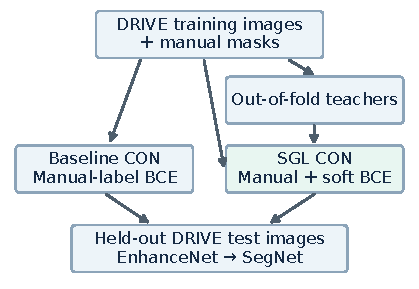
\includegraphics[width=\columnwidth]{workflow}
\caption{Paired experiment workflow. Each fold teacher produces targets for its held-out training group. Both final models use the same CON architecture and are evaluated on the same held-out DRIVE images. BCE denotes binary cross-entropy.}
\label{fig:workflow}
\end{figure}

\section{Related Work}
Staal \textit{et al.} described DRIVE and a segmentation method based on image ridges~\cite{staal}. U-Net introduced a symmetric encoder-decoder with skip connections to combine spatial detail with contextual features~\cite{unet}. The SGL reference combines two U-Nets for enhancement and segmentation and adds cross-validated soft targets during training~\cite{zhou,sglcode}. Our implementation follows this design and focuses on the effect of the added supervision on DRIVE. The published work also examines controlled label erasure and evaluates on CHASE\_DB1.


\section{Method}
\subsection{Shared Architecture}
An RGB image passes through EnhanceNet, a U-Net that yields a three-channel learned representation. SegNet, a second U-Net, converts that representation to a single probability map. Each encoder has four downsampling stages, with skip connections to the corresponding decoder levels. EnhanceNet divides the RGB input by 255. The loss supervises the output of SegNet and its gradients also train EnhanceNet. The implementation contains 15,533,320 trainable parameters. Both arms share the inference architecture (Fig.~\ref{fig:workflow}).

\subsection{Out-of-Fold Supervision}
Let \(T\) be the training set and let \(T_1,\ldots,T_K\) be disjoint groups whose union is \(T\). Teacher \(M_k\) is trained on \(T\setminus T_k\) with manual labels. For image \(x_i\in T_k\), the soft target is \(q_i=M_k(x_i)\). Each training image receives one map. The implementation stores maps as 8-bit PNGs and rescales them to \([0,1]\) during final training.

With manual target \(y_i\) and final prediction \(p_i\), the objectives are
\begin{align}
\mathcal{L}_{\mathrm{base}} &= \operatorname{BCE}(p_i,y_i),\\
\mathcal{L}_{\mathrm{SGL}} &= \operatorname{BCE}(p_i,y_i)
+ \operatorname{BCE}(p_i,q_i).
\end{align}
The BCE terms are averaged over crop pixels. The FOV is applied during primary evaluation. A fold manifest records the study groups and training settings. If validation images are requested, the pipeline excludes them from final training and from every fold teacher's training set.

\section{Experimental Setup}
\subsection{Dataset and Preprocessing}
We use the DRIVE partition of 20 training and 20 test images~\cite{staal}. The local DRIVE files contain 565 by 584 pixel RGB photographs and corresponding FOV masks. The first manual segmentation supplies training and evaluation targets. The second manual annotation for each test image provides an independent observer for the agreement analysis.

During training, random square patches undergo horizontal and vertical flips and transposition with aligned image and target transforms. For teacher inference and evaluation, full images are padded on the bottom and right to 608 by 608. Predictions are cropped back before scoring. The images remain at their native sampling resolution.

\begin{table}[!t]
\caption{Pilot and Planned Full-Run Settings}
\label{tab:config}
\centering\footnotesize
\begin{tabular}{@{}lcc@{}}
\toprule
Setting & CPU pilot & Colab GPU plan \\
\midrule
Study groups \(K\) & 2 & 8 \\
Epochs per teacher & 3 & 15 \\
Epochs per final model & 5 & 25 \\
Patch size (pixels) & 96 & 256 \\
Patches/image/epoch & 8 & 40 \\
Batch size & 4 & 4 \\
Adam learning rate & \(10^{-4}\) & \(10^{-4}\) \\
Affine/elastic augmentation & Off & On \\
Inference variants & 1 & 8 \\
Checkpoint rule & Last epoch & Last epoch \\
\bottomrule
\end{tabular}
\end{table}

\subsection{Fixed-Budget Pilot}
The CPU pilot uses seed 0, two non-overlapping groups of ten training images, and the settings in Table~\ref{tab:config}. The final models share the seed, optimizer, number of training patches, augmentation and checkpoint rule. Both use all 20 training images and evaluate the fixed fifth checkpoint without consulting test labels for selection. Binary masks use the shared threshold \(p>100/255\).

\subsection{Metrics and Paired Analysis}
We compute sensitivity, specificity, accuracy, ROC-AUC, Dice, and vessel intersection over union (IoU) separately inside each image's FOV, then take the unweighted mean. ROC-AUC uses model probabilities. The other metrics use binary masks. Dice is \(2TP/(2TP+FP+FN)\), so an all-background prediction can have high accuracy and zero vessel overlap.

For each metric we subtract the baseline score from the SGL score on the same image. Empirical 95\% percentile intervals resample the 20 images as pairs with replacement using 10,000 draws and seed 2026. These intervals reflect test-image variation conditional on the two fitted models. Training-seed variation remains unmeasured.

\begin{figure*}[!t]
\centering
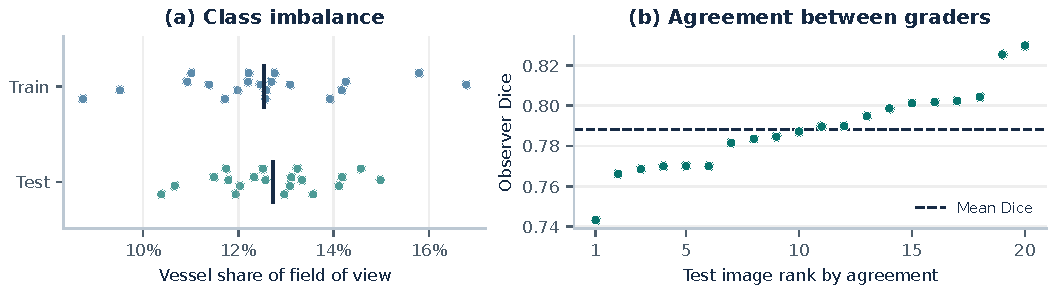
\includegraphics[width=0.98\textwidth]{drive_data}
\caption{DRIVE data audit. (a) In-FOV vessel fraction in the first manual mask of each image. Vertical ticks mark the split means. (b) Agreement between the two manual masks, sorted by Dice. Each marker represents one image.}
\label{fig:drive}
\end{figure*}

\section{Results and Discussion}
\subsection{Dataset Audit}
Vessels occupied a mean of 12.54\% of the training FOV and 12.73\% of the test FOV. Treating all test pixels as background would yield 87.27\% accuracy and zero vessel Dice. The two test annotations had mean Dice 0.7881 (range 0.7433 to 0.8298) and disagreed on a mean of 5.27\% of in-FOV pixels. Figure~\ref{fig:drive} shows the image-to-image variation. The observer comparison describes agreement with the first grader. The correct label at individual disputed pixels remains unresolved.

\begin{table}[!t]
\caption{Paired Pilot Results on DRIVE (Mean per Image, Inside FOV)}
\label{tab:pilot}
\centering\footnotesize
\begin{tabular}{@{}lrrr@{}}
\toprule
Metric & Baseline & SGL & Change (pp) \\
\midrule
Accuracy & 0.12740 & 0.12730 & \(-0.0101\) \\
Sensitivity & 0.99994 & 1.00000 & \(+0.0062\) \\
Specificity & 0.00013 & 0.00000 & \(-0.0126\) \\
ROC-AUC & 0.91033 & 0.91778 & \(+0.7455\) \\
Dice / F1 & 0.22566 & 0.22565 & \(-0.0009\) \\
Vessel IoU & 0.12731 & 0.12730 & \(-0.0006\) \\
\bottomrule
\end{tabular}
\end{table}

\subsection{Paired Pilot Results}
At the fixed threshold, SGL marked every in-FOV pixel as vessel. The baseline marked almost as many. Sensitivity was near one and specificity was near zero for both (Table~\ref{tab:pilot}). Dice and vessel IoU remained effectively unchanged, so the observed masks did not support the expected trade-off.

ROC-AUC increased by 0.75 percentage points (paired 95\% interval, 0.24 to 1.21 points) and rose in 16 of 20 images (Fig.~\ref{fig:effects}). The improvement shows better ranking of vessel relative to background scores in this pilot. The low specificity shows that the shared threshold did not turn that ranking into useful masks.

\begin{table}[!t]
\caption{Published DRIVE Reference From Zhou et al.~\cite{zhou}, Appendix Table~3}
\label{tab:reference}
\centering\footnotesize
\begin{tabular}{@{}lrr@{}}
\toprule
Metric & Published baseline & Published SGL (\(K=8\)) \\
\midrule
Accuracy & 0.9695 & 0.9705 \\
Sensitivity & 0.8341 & 0.8380 \\
Specificity & 0.9827 & 0.9834 \\
ROC-AUC & 0.9867 & 0.9886 \\
Dice / F1 & 0.8262 & 0.8316 \\
Vessel IoU & 0.7041 & 0.7120 \\
\bottomrule
\end{tabular}
\end{table}

\subsection{Published Reference}
Table~\ref{tab:reference} lists the published scores at the original training label ratio. Zhou \textit{et al.} report a sensitivity increase of 0.39 percentage points and a Dice increase of 0.54 points for their full eight-group setting. The training schedule, teacher quality, augmentations, and evaluation protocol can affect the comparison. Our pilot measures the paired change under the settings in Table~\ref{tab:config}.

\begin{figure*}[!t]
\centering
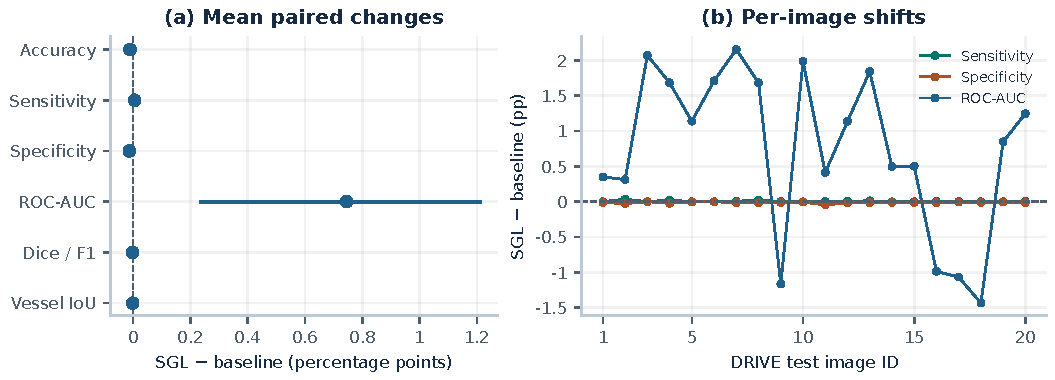
\includegraphics[width=0.98\textwidth]{pilot_effects}
\caption{Effects of SGL in the CPU pilot. (a) Mean SGL-minus-baseline changes with paired 95\% bootstrap intervals. (b) Differences on each image for sensitivity, specificity, and ROC-AUC. Positive values indicate a higher metric for SGL.}
\label{fig:effects}
\end{figure*}

\section{Failure Analysis}
We align both predictions and the first manual mask within the FOV. For reference vessel pixels, a recovery is a baseline miss detected by SGL. A new miss is a baseline detection lost by SGL. For reference background pixels, a removal is a baseline false positive that becomes background under SGL. A new false vessel is created when SGL predicts vessel where the baseline correctly predicted background. Shared errors occur when both arms disagree with the first grader.

\begin{table}[!t]
\caption{Pooled Paired Error Counts Across 20 Test Images}
\label{tab:errors}
\centering\footnotesize
\begin{tabular}{@{}lrrr@{}}
\toprule
Pixel error & Shared & Removed by SGL & Added by SGL \\
\midrule
Missed vessel & 0 & 38 & 0 \\
False vessel & 3,959,997 & 0 & 497 \\
\bottomrule
\end{tabular}
\end{table}

SGL recovered the baseline's 38 missed vessel pixels and introduced 497 false vessel pixels (Table~\ref{tab:errors}). Both models shared nearly four million false vessel pixels. The pooled counts explain why the sensitivity increase had little practical value at this operating point.

Figure~\ref{fig:errors} shows that vessel scores tend to be higher than background scores despite the threshold being below nearly all of both distributions. The lowest saved SGL score was 0.396 after 8-bit quantization, above the fixed threshold of 0.392. The shared false-positive map pools counts on a common grid in image coordinates, where no anatomical alignment is assumed.

A branch-level analysis could stratify results by vessel caliber and quantify fragmentation. The current analysis treats pixels equally and cannot establish whether recovered pixels restore continuous branches. Reviewing both manual masks would help interpret ambiguous areas.

\begin{figure*}[!t]
\centering
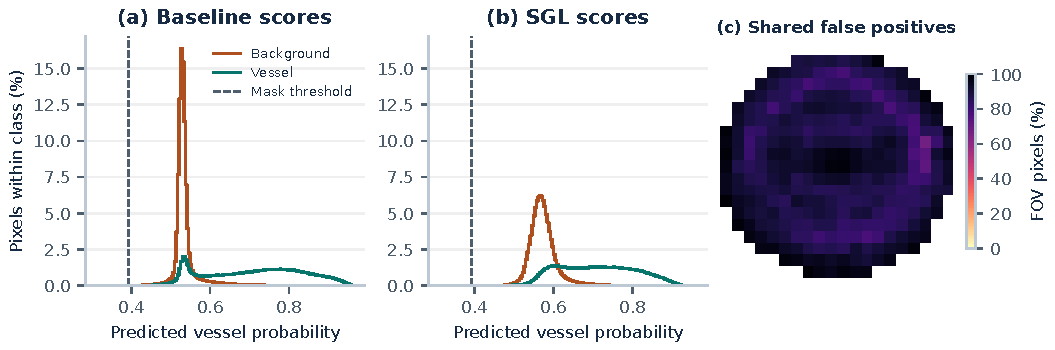
\includegraphics[width=0.98\textwidth]{operating_point}
\caption{Failure at the fixed operating point. (a--b) Pooled distributions of the saved 8-bit vessel scores, normalized within each manual class. (c) Shared false positives as a percentage of in-FOV pixels per cell on a 20-by-20 image grid. Cells with fewer than 500 FOV pixels are omitted.}
\label{fig:errors}
\end{figure*}

\section{Limitations}
The pilot uses one seed, two study groups, three teacher epochs, and five final epochs. Early teacher predictions can carry systematic omissions or weakly separated scores into the SGL objective. Masks use one fixed operating point. Alternative thresholds require an independent validation procedure.

The 20 test images come from one dataset. Pixel errors within each image are spatially dependent, so we resample images and report pooled pixel counts descriptively. The experiment covers the original annotations only. Generalization to other datasets and the effect of controlled label erasure are open questions for this implementation.

\section{Conclusion}
The reproduction implements paired manual-label and out-of-fold supervision on DRIVE. The data audit and paired error maps make the operating-point behavior interpretable alongside accuracy and ROC-AUC. The reduced training run improved score ranking with SGL, but both arms produced nearly all-vessel masks at the specified threshold. A full eight-group run, independent threshold validation, and multiple seeds are needed to assess the sensitivity-specificity hypothesis.

\section*{Reproducibility}
The project repository provides the PyTorch pipeline, a Colab GPU notebook, CPU pilot instructions, an analysis script, and per-image and summary statistics. Report figures use derived and aggregate data. DRIVE is available separately from its original distribution. Artifacts are available at \href{https://github.com/A-cpu-rg/Retinal-vessel-segmentation-sgl}{the project repository}.

\IEEEtriggeratref{3}
\begin{thebibliography}{00}
\bibitem{zhou}
Y. Zhou, H. Yu, and H. Shi, \textquotedblleft Study Group Learning: Improving retinal vessel segmentation trained with noisy labels,\textquotedblright\ in \emph{Proc. MICCAI}, 2021. [Online]. Available: \url{https://arxiv.org/abs/2103.03451}

\bibitem{staal}
J. Staal, M. D. Abràmoff, M. Niemeijer, M. A. Viergever, and B. van Ginneken, \textquotedblleft Ridge-based vessel segmentation in color images of the retina,\textquotedblright\ \emph{IEEE Trans. Med. Imag.}, vol. 23, no. 4, pp. 501--509, 2004, doi: \href{https://doi.org/10.1109/TMI.2004.825627}{10.1109/TMI.2004.825627}.

\bibitem{unet}
O. Ronneberger, P. Fischer, and T. Brox, \textquotedblleft U-Net: Convolutional networks for biomedical image segmentation,\textquotedblright\ in \emph{Proc. MICCAI}, 2015, pp. 234--241. [Online]. Available: \url{https://arxiv.org/abs/1505.04597}

\bibitem{sglcode}
SHI Labs, \textquotedblleft SGL-Retinal-Vessel-Segmentation,\textquotedblright\ reference implementation. [Online]. Available: \href{https://github.com/SHI-Labs/SGL-Retinal-Vessel-Segmentation}{GitHub repository}.
\end{thebibliography}
\end{document}
